\documentclass{report}

\usepackage{suthesis-2e}

%standard packages
\usepackage{graphicx}
\usepackage{color}
% \usepackage{hyperref}

%misc atlas packages and helper packages
\usepackage{atlasbsm}
\usepackage{atlasmisc}
\usepackage{atlasunit}
\usepackage{jetetmisssymbols}
\usepackage{boostedsymbols}
\usepackage{susysymbols}
\usepackage{edittools}


\graphicspath{{figures}{figures/detector/}{figures/lhc}}

\dept{Physics}


\begin{document}
\title{Measuring the Standard Model and Searching for New~Physics 
        With Jet Substructure Using the ATLAS Detector}
\author{Maximilian Swiatlowski}
\principaladviser{Ariel Schwartzman}
\firstreader{Su Dong}
\secondreader{Jay G. Wacker}
\thirdreader{Blas Cabrera (???)} %if needed
\fourthreader{???} %if needed

 
\beforepreface
\prefacesection{Preface}
    This thesis tells you all you need to know about...
\prefacesection{Acknowledgments}
    I would like to thank...
\afterpreface
 
\chapter{Introduction}
         ...

\chapter{The Standard Model, and the Theory of Strong Interactions}
		 ...

\chapter{Supersymmetry, $R$-Parity, and Naturalness}
		 ...


\chapter{The Large Hadron Collider}
%!TEX root = ../swiatlow_thesis.tex
\label{chapter:lhc}

The Large Hadron Collider (LHC) is a 27 km long proton-proton ($pp$) synchotron built on the border of France and Switzerland, near the city of Geneva. The accelerator is nestled beneath mostly bucolic French farmland, as seen in Figure~\ref{fig:lhc:cern-lhc-aerial}. The total costs of the accelerator and the detectors it serves are estimated at \$20 billion, making the LHC one of the largest scientific enterprises ever attempted. \editnote{cite this} The project is full of similar superlatives: the accelerator is the largest machine, the ATLAS detector is the largest detector, the CMS detector is the heaviest. 10,000 scientists from 113 countries work on some aspect of the project, making it one of the best examples of international cooperation that mankind has produced.

%%%%%%%%%%%%%%%%

\begin{figure}
\centering
\includegraphics[width=0.8\textwidth]{cern-lhc-aerial.jpg}
\label{fig:lhc:cern-lhc-aerial}
\caption{An aerial view of Geneva, with the location of the LHC superimposed. The individual detectors (described in chapter~\ref{chapter:detector}, as well as the main CERN Meyrin site, are also highlighted. Image courtesy CERN.}
\end{figure}

%%%%%%%%%%%%%%%% 

The design of the machine aims to deliver collisions at $\sqrt{s} = 14$~\TeV~energy at a rate of $10^{34}$~\lumirate-- an energy at which protons in the LHC will be moving at 99.9999991$\%$ the speed of light, and where the beams will contain as much energy as a 38 ton truck traveling at 500 km/h.  As of 2012 collisions had only occured at 8 \TeV and a rate of $5\times10^{33}$~\lumirate-- enough to discover the Higgs Boson, but not yet enough to discover physics beyond the standard model.

The following sections describe first the history of the LHC project, followed by the details of the machine design, luminosity considerations, and operations during 2010-2012.

\section{History}
\label{lhc:history}

The LHC was first discussed publically at the ECFA-CERN Workshop held at Lausanne and Geneva in March of 1984~\cite{ECFA1984}\footnote{4 years and 1 month before the author was born!}. This was a very active time for proposing new collider experiments, as extensive work on the 40~\TeV $pp$ Superconducting Supercollider (to be built in Waxahachie, Texas) had recently displaced a proposal for a 4~\TeV~$p\bar{p}$ Dedicated Collider at Fermilab~\cite{ECFA1984,DC}, though construction continued on Fermilab's 2~\TeV~$p\bar{p}$ Tevatron collider. The Soviet Union was even planning a 6~\TeV~$p\bar{p}$ collider, the Accelerator and Storage Complex (UNK)~\cite{UNK}\editnote{This needs a better citation}. In this busy landscape, the proposal of another machine at CERN-- which was currently building the Large Electron Positron (LEP), the world's largest $e^+/e^-$ collider-- was very ambitious indeed.

Several characteristics made the proposed LHC unique and worth pursuing in such a competitive environment. First, with the construction of the LEP tunnel on track for completion in 1988, the civil-engineering component of the project was greatly reduced, especially compared to the enormous expense of constructing the SSC tunnel. Second, while the design goals of 20~\TeV~collisions were at a significantly lower energy than the SSC, the projected luminosity was eventually designed to be a factor of 10 higher (10$^{34}$~\lumirate, though the initial designs focused on 10$^{33}$~\lumirate) and so the LHC could potentially gain sensitivity by accumulating data more quickly. Finally, as figure \ref{fig:lhc:lep-lhc} shows, the initial designs for the LHC invisaged the LHC beamlines actually sitting on top of the existing LEP beamlines. The resulting hybrid collider would be able to run $pp$, $ep$, and $ee$ collisions. This would not only extend the reach of the physics program by allowing for the study of deep inelastic scattering at higher energies than the HERA collider at DESY \editnote{Cite this-- HERA and $e/p$ if possible.}, but would also allow for the study of $Z$ bosons from $ee$, which could potentially be used as a calibration source for detectors before $pp$ collisions~\cite{ECFA1984}.

%%%%%%%%%%%%%%%%

\begin{figure}
\centering
\includegraphics[width=0.8\textwidth]{lep-lhc.pdf}
\label{fig:lhc:lep-lhc}
\caption{A schematic drawing of the initial design of a shared LEP/LHC tunnel, with the LHC beamline positioned on top of the existing LEP beamline~\cite{ECFA1984}.}
\end{figure}

%%%%%%%%%%%%%%%% 

With the approval of the SSC in 1987 and the subsequent start of construction in 1991, CERN was mostly focused on the construction and operation of LEP but did not stop planning for the LHC. This proved remarkly prescient, as in the face of changing budget priorities and the end of the Cold War, the SSC ended up being cancelled in 1993. \editnote{This probably needs citations.} CERN, on the other hand, approved a staged construction plan for the LHC in 1994, targetting first 10~\TeV~collisions in 2004 and then a higher energy in 2008. \editnote{Statement about internation collaboration, compared to SSC? Statement about the 10 TeV plan being dropped?}

The Conceptual Design Report~\cite{LHCCDR} published in 1995 reflected the changed landscape with the demise of the SSC and the results of more detailed cost estimates. The design energy was lowered to 14~\TeV-- higher energies would have required more costly magnets-- while the design luminosity was actually increased to 10$^{34}$~\lumirate. This increase in luminosity came at a cost: the number of interaction points was reduced to four instead of eight, and only two would receive collisions at a high rate. \editnote{Mention pileup here or no?} Critically, it was also decided to remove the LEP beamline and magnets, as it was deemed too costly to follow the existing LEP infrastructure. While this reduced the physics program of the LHC, being the only high energy hadron collider was still a rather broad portfolio. For budgetary reasons, the initial proposal was for a two-stage design, with the first stage operating with only two-thirds the dipoles and therefore a lower energy.

Non-member states joined the proposal quickly: Japan contributed in 1995; India, Russia, and Canada joined in 1996; and the US became a partner in 1997. This financial outlook for the LHC was still not completely safe, as Germany (and later the UK) unilaterally reduced their contribution to CERN between 8-9$\%$. This issue was resolved by allowing CERN to take on debt to finance the entire project in one construction phase-- a decision which raised the total cost of the LHC by $20\%$.


With the shutdown of LEP in 2001\footnote{Not without controversy, as there was perhaps a tantalizing sign of an excess in Higgs-boson like events during the final runs of LEP.\editnote{cite me}}, the construction of the LHC began in earnest. It would take till 2007 to install the last magnet in the LHC, and the detectors finalized their own installations only in 2008. Figure~\ref{fig:lhc:lhc-tunnel} shows the final state of the LHC tunnel (without the originally planned LEP beamline). The first low-energy collisions occured on September 10, 2008, putting the LHC almost on track of its initial goal of 14~\TeV collisions in 2008. \editnote{Probably want to add a bit more on construction.}

%%%%%%%%%%%%%%%%

\begin{figure}
\centering
\includegraphics[width=0.8\textwidth]{lhc-tunnel.jpg}
\label{fig:lhc:lhc-tunnel}
\caption{A photo of the final LHC tunnel, no LEP beamline, in contrast to the first plans shown in Figure~\ref{fig:lhc:lep-lhc}. Photo courtesy of USLHC.}
\end{figure}

%%%%%%%%%%%%%%%% 

However, an ``incident'' on September 19 ended up delaying the full startup for a year~\cite{Incident}. On that day, the operators were testing the last sector of the LHC at current levels appropriate fo 5.5~\TeV beams. A resistive zone developed in the electrical bus connection between a dipole and quadrupole magnet. While the power supply detected this and shut down within 0.39 seconds and the quench protection circuitry began to engage at 0.89 seconds, it was already too late: an electrical arc had sparked and punctured the liquid helium enclosure and the insulation vacuum along the cryostat. This, along with the electrical noise induced by the power supply shutdown and the heat dissipation caused by the quench protection circuitry, triggered a chain reaction in which several other magnets also began to quench and other vacuum systems were degraded. As the helium began to escape the cryostat, pressure relief valves correctly opened and vented the helium to atmosphere. However, an additional complication proved to be a problem: neighboring subsectors had their vacuum systems separated by vacuum barriers, meant to isolate the vacuum systems of neighboring areas. The vacuum barriers could only sustain a rather low pressure difference, and the extreme pressures generated by the evacuating helium overwhelmed these connections. The attendant large pressure forces ended up displacing dipoles from their support structures, and knocked the cryostats from their support jacks-- in some cases even ripping the anchors from the concrete floor. A total of six tons of helium, five quadrupoles, and twenty-four dipoles were lost in the incident. 

The damage to the accelerator was repaired in 2009, and on November 20, 2009, 450 GeV protons from the Super Proton Synchotron were injected into the LHC for the first time since the incident. November 23rd saw the first $pp$ collisions in all four LHC detectors, albeit at only $\sqrt{s} = 900$~\GeV. Several very short runs at this energy and $\sqrt{s} = 2.36$~\TeV followed, before the first $\sqrt{s} = 7$~\TeV collisions occured on March 30, 2010. It was decided to operate the LHC for several years at this lower energy, as more accelerator upgrades and consolidation would be required to safely operate at $\sqrt{s} = 14$~\TeV. 2010 saw a peak luminosity of only $2\times10^{32}$~\lumirate as the accelerator only very gradually increased the collision rate. 2011 saw delivery at a peak of $4 \times 10^{33}$~\lumirate-- only three times lower than the design luminosity.

After two years of successful and safe operations at the reduced energy, 2012 saw a large increase in luminosity-- to a peak of $8\times10^{33}$~\lumirate-- and an increase of the collision energy to 8~\TeV. The LHC then proceeded to shut down in 2013 until mid-2015 for a further round of repairs and consolidations of electrical connections to guarantee the safety of operations at near the design energy. As the restart of the LHC approaches in the coming months, we are anticipating collisions at 13~\TeV with luminosity likewise reaching near design levels. The LHC will have broken energy records twice in the span of five years, making this an incredibly exciting time to be working in particle physics.


\section{Machine Design}

The LHC is the last of a long chain of accelerators used to accelerate ordinary protons obtained from hydrogen gas\cite{cern-accelerators}. The entire accelerator complex is shown in Figure~\ref{fig:lhc:cern-accelerators}. Protons from a simple bottle of hydrogen gas are stripped of their electrons in an electric field and are injected into the chain at the Linac2, which accelerates the particles to 50 MeV. The Proton Synchotron Booster (PSB) then accelerates the particles to 1.4 GeV, and sends them off to the Proton Synchotron (PS) to be accelerated to 25 GeV. The Super Proton Synchotron (SPS) then accepts the protons and accelerates them to 450 GeV, which is the energy of injection at the LHC. The injection process per beam takes 260 seconds, and then another 20 minutes is required to raise the energy to collision levels.

%%%%%%%%%%%%%%%%

\begin{figure}
\centering
\includegraphics[width=0.8\textwidth]{cernaccelerators.jpg}
\label{fig:lhc:cern-accelerators}
\caption{A diagram of the CERN accelerator chain, with each accelerator listing both its year of completion and length. Copyright CERN.}
\end{figure}

%%%%%%%%%%%%%%%% 

Each stage of the chain accelerates particles by a factor of between 10-20 times their energy. This is a consequence of the fixed bending radius in an accelerator, $\rho$, which is~\cite{accelerator-book}:
%
\begin{equation}
\label{lhc:bending}
\frac{1}{\rho} (\mathrm{m}^{-1}) = 0.2998 \frac{|B (\mathrm{T})|}{\beta E (\GeV)}.
\end{equation}
%
As the bending radius is fixed, this means that as the energy of the beam goes up, the magnetic field must go up linearly to keep the particles inside the ring. This also means that as particles are injected from one accelerator to another (and the radius therefore increases), the magnetic field must be the same factor smaller. The lower range of practical bending magnet strength is set by stray magnetic fields in the earth; the upper range is set by the material of the magnet and energy consumption. These restrictions (how weak the magnets can be during injection, and how strong after acceleration) limit each stage of the accelerator chain to increasing the energy by a factor of $\approx$200. In practice, the accelerating factor is lower (10-20), because it is much easier to not use the full range of the magnet strength (particularly at the low end), and the size of each accelerator is not designed optimally but instead historically, as each accelerator was previously used for collisions at a lower energy. For example, the SPS could have been ejected particles at a much lower energy and the LHC accepted them by using a lower initial field strength, but as the SPS was already built, the operation of the LHC is simplified by using a higher initial field. \editnote{This might need revision}


The LHC itself is composed of eight essentially identical octants, as shown in Figure~\ref{fig:lhc:ring}. Octant 1 contains the collision point for ATLAS (conveniently located right next to the main CERN campus), and Octant 5 for CMS (located in the middle of the French countryside). Each octant is composed of an `insertion'-- a straight segment used for collisions, cleaning, acceleration, beam dumps, etc., as labelled in Figure~\ref{fig:lhc:ring}-- and one half of an `arc' on either end of the insertion point. Each pair of half-arcs forms a sector, which is the main organizational unit for the machine: each sector is independently powered and shares a continuous cryostat. The ring is composed of 1232 dipole magnets which bend the beam around the ring, and 852 quadruple magnets used for beam focusing. The strength of the dipole magnets limits the energy of the beam, as discussed in Equation~\ref{lhc:bending}, so these magnets are particularly critical to the machine design. They are constructed from Niobium-Titanium wire and operated at a temperature of 1.9 K (provided by superfluid helium cooling) at a strength of 8.3 T, using 11850 A of current. An additional 7000 smaller correction magnets (with sextuple, octupole, etc. configurations) are used to shape the beam. The acceleration of the beam is performed by 8 super-conducting RF cavities per beam, each providing an acceleration gradient of 5 MV/m at 400 MHz. 

Operating at full design luminosity, each beam of the LHC contains 2808 bunches each filled with $10^{11}$ protons. This corresponds to a bunch spacing of 25 ns, with longer spacing in between so-called ``bunch trains'': the exact structure of the fill pattern is determined by the fill patterns of the prior accelerators, and the need to provide gaps which can be used to safely dump the beam if necessary~\cite{lhc-bunches}\footnote{In particular, the size of these gaps is determined by the turn-on time of the LHC beam dump kicker of about 3~$\mu$s.}. In operations in 2010-2012, a minimum bunch spacing of 50 ns was used due to electron-cloud effects restricting the operation at 25 ns; the bunch charge was instead increased to deliver additional luminosity. 

emmittance, etc.

stored beam energy

table summarizing parameters

%%%%%%%%%%%%%%%%

\begin{figure}
\centering
\includegraphics[width=0.8\textwidth]{ring.png}
\label{fig:lhc:ring}
\caption{A diagram of the CERN accelerator chain, with each accelerator listing both its year of completion and length. Copyright CERN.}
\end{figure}

%%%%%%%%%%%%%%%% 

\section{Luminosity, and Pileup}
\label{lhc:luminosity-and-pileup}


%%%%%%%%%%%%%%%%

\begin{figure}
\centering
\includegraphics[width=0.7\textwidth]{mu_2011_2012-dec.pdf}
\label{fig:lhc:mu-profile}
\caption{muuu}
\end{figure}

%%%%%%%%%%%%%%%% 


\section{Operations in 2010-2012}

some more lumi plots? instaneous?

pileup plots (or is that earlier)



%%%%%%%%%%%%%%%%

\begin{figure}
\centering
\includegraphics[width=0.7\textwidth]{lumivstime.pdf}
\label{fig:lhc:lumivstime}
\caption{lumi vs time}
\end{figure}

%%%%%%%%%%%%%%%% 


%%%%%%%%%%%%%%%%

\begin{figure}
\centering
\includegraphics[width=0.7\textwidth]{muvstime.pdf}
\label{fig:lhc:lumivstime}
\caption{mu vs time}
\end{figure}

%%%%%%%%%%%%%%%% 


%%%%%%%%%%%%%%%%

\begin{figure}
\centering
\includegraphics[width=0.7\textwidth]{intlumivsyear.pdf}
\label{fig:lhc:lumivsyear}
\caption{lumi vs year}
\end{figure}

%%%%%%%%%%%%%%%% 
		

\chapter{The ATLAS Detector}
%!TEX root = ../swiatlow_thesis.tex
\label{chapter:detector}

The design of the LHC, with two high-luminosity interaction points at opposite ends of the ring, called for two general purpose detectors to be built in these locations. Their charge was to accurately reconstruct collision events in the most hostile conditions yet seen in a collider: with a bunch spacing of 25 ns and the unprecedented introduction of pile-up the detectors would have an enormous challenge ahead of them in dealing with both the rate and the reconstruction of events. ATLAS (A Toroidal LHC APparatus)~\cite{ATLASPaper} and CMS (Compact Muon Solenoid)~\cite{CMSPaper} were the two detectors built for this task, with ATLAS occupying the (much more convenient) Point 1 and CMS located at the (very distant) Point 5. The data presented in this thesis was collected by the ATLAS experiment in $pp$ collisions at $\sqrt{s} = 8$~TeV in 2012. 


\editnote{Paragraph on general principles?}


Particle detectors measure particles via their interactions with matter, as drawn schematically in Figure~\ref{fig:detector:schematic}. For example, charged particles (such as electrons and some hadrons) interact electromagnetically with silicon and gas tubes, leaving hits in different layers of detectors which can be traced back to form a track. Electrons and photons, with their low masses and high rate of interaction with matter, are measured by the electromagnetic calorimeter. The calorimeter is composed of alternating layers of metal meant to cause the particle to interact and lose energy, and active materials which measure the energy left behind in these interactions. The hadron calorimeter follows a similar principle, and alternately placed layers of metal and active material again aim to stop and measure the hadrons which the electromagnetic calorimeter did not stop. Muons, which do not interact very much with matter most matter but do leave hits in trackers, survive past even the hadronic calorimeter, and a special set of muon detectors can be used to identify them there. Neutrinos, as they interact with matter only via the weak force and thus very rarely, escape detection and are reconstructed only by inferring their presence from the lack of momentum conservation in the transverse plane. \editnote{this isn't great?}


%%%%%%%%%%%%%%%%

\begin{figure}
\centering
\includegraphics[width=0.7\textwidth]{schematic.jpg}
\label{fig:detector:schematic}
\caption{A schematic diagram of the interactions of various particles with detector components. Copyright CERN.}
\end{figure}

%%%%%%%%%%%%%%%% 

General purpose particle detectors thus demand the following characteristics: \editnote{define radiation lengths? above?}

\begin{enumerate}
	\item Tracking systems must be able to identify primary and secondary vertices, while minimizing the radiation lengths before the calorimeters
	\item Strong calorimetry systems are required to accurately measure the energy and position electrons, photons, and hadrons
	\item Muon systems must be able to precisely reconstruct muons
\end{enumerate}

To this end, the ATLAS detector is built in the traditional onion-layer configuration, which measures particles as they travel perpendicular to the beam. The Inner Detector, composed of the concentric Pixel, SCT \editnote{define}, and Transition-Radiation-Tracker (TRT) subsystems, lies at the center of the detector and precisely measures tracks created by charged particles. A 2 T solenoid encloses the Inner Detector, bending charged particles and enabling the measurement of their momenta. Next the Electromagnetic Calorimeter (ECal), composed of liquid argon (LAr) and copper, sits outside of the solenoid in a liquid nitrogen cryostat, and measures energy deposits from electrons and photons (as well as hadrons to a lesser extent). The Hadronic Calorimeter, built to measure and stop any remaining hadronic particles, is composed of steel and scintillating tile in the center (referred to as the barrel), and LAr and copper in forward regions (referred to as end-caps). Surrounding these are an additional set of magnets: the superconducting air-core toroids of the barrel and endcaps, which bend particles in the plane perpendicular to that of the bending due to the solenoid. \editnote{That needs cleaning.} The Muon Spectrometer (composed of MDT, RPC, TGC, and CSC subsystems) sits outside of (and next to) these magnets, and provides a final measurement of the charged particles which reach that far. The entire detector is shown in Figure~\ref{fig:detector:atlas}. The incredible size of the detector-- 25 m in diameter, and 46 m long-- is dominated by the Muon Spectrometer and the toroids. On the other hand, the detector is comparatively light (only 7000 tons, compared to 14,000 tons for CMS), as the air-core toroids do not add substantial weight to the detector. \editnote{decide how to cite all this}


%%%%%%%%%%%%%%%%

\begin{figure}
\centering
\includegraphics[width=0.85\textwidth]{atlas.jpg}
\label{fig:detector:atlas}
\caption{A computer-generated view of the ATLAS detector, with people for scale. Copyright CERN.}
\end{figure}

%%%%%%%%%%%%%%%% 


In keeping with the principle of ``similar, but opposite'' established by their locations, the ATLAS and CMS detectors take complementary approaches to the various aspects of event reconstruction in collisions. All general purpose detectors have the same basic goals: the must reconstruct the outgoing, stable particles produced in collisions and the subsequent decays of particles in these collisions. Different particles are detected with different general classes of detectors, of which there are many possible types. For example, electrons and photons are measured by the ECal, for which ATLAS used a liquid argon (LAr) and copper system while CMS used a crystal lead tungstate system. Each had their own advantages and disadvantages (ATLAS's was less costly and already proven technology with better position resolution, while CMS took a riskier route which promised better energy resolution), but overall performance between the detectors tends to be very similar because of various trade-offs. In the case of the ECals, the precision of ATLAS and CMS's $H\rightarrow \gamma \gamma$ measurements ended up being largely similar \editnote{cite?}, in no small part because CMS's all-silicon tracking system introduced greater radiation lengths before the calorimeters, thereby prompting more photons to convert and losing precision in the measurement. On the other hand, CMS's comparatively weak brass hadronic calorimeter (compared to ATLAS's higher resolution tile calorimeter), is compensated by their tracking system, which enables a particle-flow reconstruction algorithm to combine information from all detectors and improve jet performance to levels very similar to ATLAS. \editnote{consider citations, and substantial revisions here}. Similarly, the large size and extra toroid magnets of ATLAS allow for a larger lever-arm and an additional set of measurements of muons (enabling reconstruction with or without the inner detector): however, muon reconstruction performance in CMS is very similar because the stronger solenoidal magnetic field (4 T compared to 2 T) allows for a better measurement using the inner detector only (with the muon systems on CMS providing only a tag of a passing muon, and not a complete reconstruction). 


%2012 luminosity figure? Or in LHC section?



%Detector figure

\section{History}

The first public discussion of the proposals which became the ATLAS detector occurred in 1992 at the General Meeting on LHC Physics at Evian-les-Bains~\cite{Evian,EvianCourier}. At the time, four general purpose detectors (much like the four detector configuration in place at LEP) were seriously considered: EAGLE, ASCOT, CMS, and L3 (as an upgrade to the existing LEP detector, including a movable stage which would allow it to take data from both $e^+/e^-$ and $pp$ collisions). Several additional single purpose (heavy ion, neutrino, and $B$-physics) detectors were also proposed.

ATLAS emerged in a later 1992 Letter of Intent as a merger of the ASCOT and EAGLE collaborations~\cite{ATLAS-LoI}. ASCOT (Apparatus with SuperCOnducting Toroids) contributed the physically-defining feature of the secondary toroidal magnet system and standalone muon measurement system, as well as the tradition of using a tortured amalgamation of letters to form a name. EAGLE (Experiment for Accurate Gamma, Lepton and Energy measurements) on the other hand featured a stronger 2 T magnetic field, and inner-detector and calorimeter designs more similar to some of the final ATLAS systems. The detector described in the Letter of Intent already resembled ATLAS in many important ways, featuring the superconducting air-core toroids, accordion-shaped liquid Argon electromagnetic calorimeters, scintillating tile hadron calorimeters, and multi-design inner detector. \ref{fig:detector:earlyatlas} shows an early drawing of ATLAS from the Letter, and already the detector looks recognizable to its current form.

% Any citations on UA1 origins?

%%%%%%%%%%%%%%%%

\begin{figure}
\centering
\includegraphics[width=0.7\textwidth]{early-atlas.pdf}
\label{fig:detector:earlyatlas}
\caption{An early view of a potential superconducting air-core toroid magnet system for the ATLAS detector from the 1992 Letter of Intent~\cite{ATLAS-LoI}.}
\end{figure}

%%%%%%%%%%%%%%%% 


% approval dates

% cavern construction (picture?)

% construction milestones

% first data, first papers

% quenching? higgs discovery


\section{Magnet Systems}

\subsection{Solenoid}

%%%%%%%%%%%%%%%%

\begin{figure}
\centering
\includegraphics[width=0.7\textwidth]{solenoid.jpg}
\label{fig:detector:solenoid}
\caption{A photograph of the ATLAS solenoid shortly after the winding of the coils was finished. Copyright CERN.}
\end{figure}

%%%%%%%%%%%%%%%% 


\subsection{Toroids}


%%%%%%%%%%%%%%%%

\begin{figure}
\centering
\includegraphics[width=0.7\textwidth]{toroid.jpg}
\label{fig:detector:solenoid}
\caption{A photograph of the ATLAS barrel toroids after their installation. Note person in the center for scale. Copyright CERN.}
\end{figure}

%%%%%%%%%%%%%%%% 



%%%%%%%%%%%%%%%%

\begin{figure}
\centering
\includegraphics[width=0.7\textwidth]{endcap-toroid.jpg}
\label{fig:detector:solenoid}
\caption{A photograph of an ATLAS endcap toroid shortly before its installation in the detector. Copyright CERN.}
\end{figure}

%%%%%%%%%%%%%%%% 


\section{Inner Detector}


Define ID

At design luminosity, the detector is expected to measure approximately 1000 charged particles every 25 ns within the detector acceptance.

%%%%%%%%%%%%%%%%

\begin{figure}
\centering
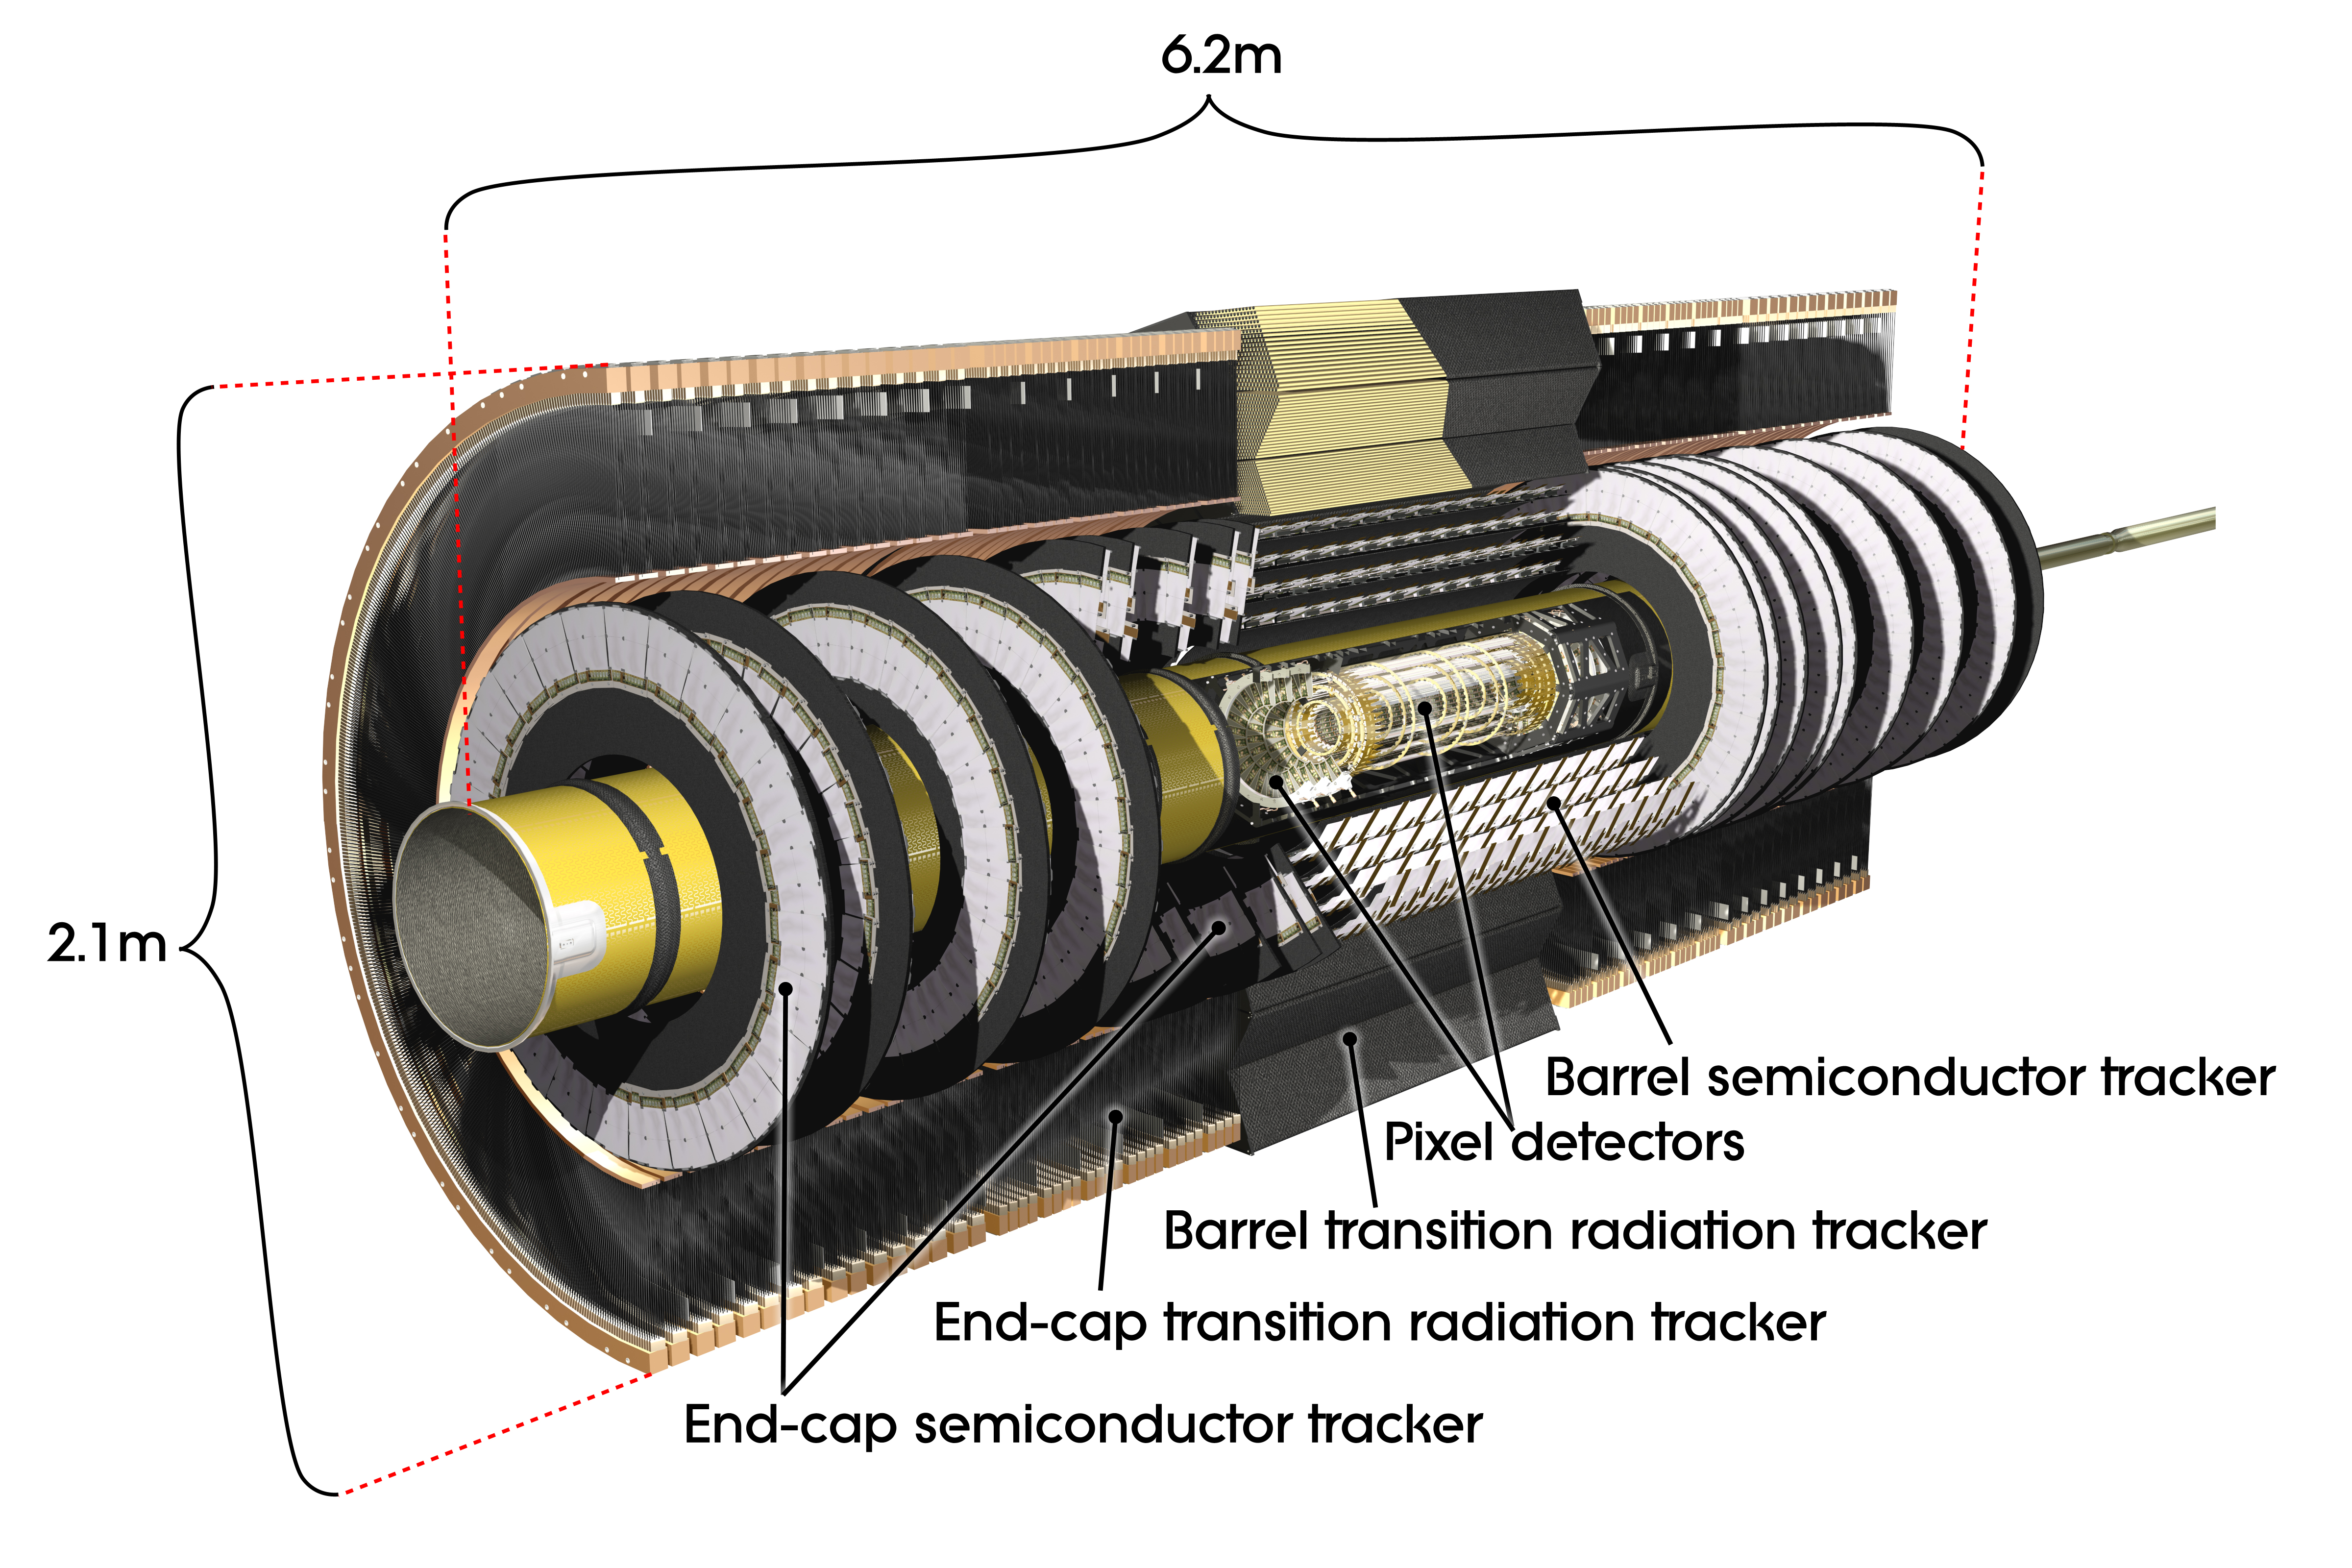
\includegraphics[width=0.7\textwidth]{inner-detector.jpg}
\label{fig:detector:inner-detector}
\caption{A computer-generated view of the ATLAS inner detector, with relevant sizes of the detector marked out. Copyright CERN.}
\end{figure}

%%%%%%%%%%%%%%%% 

%%%%%%%%%%%%%%%%

\begin{figure}
\centering
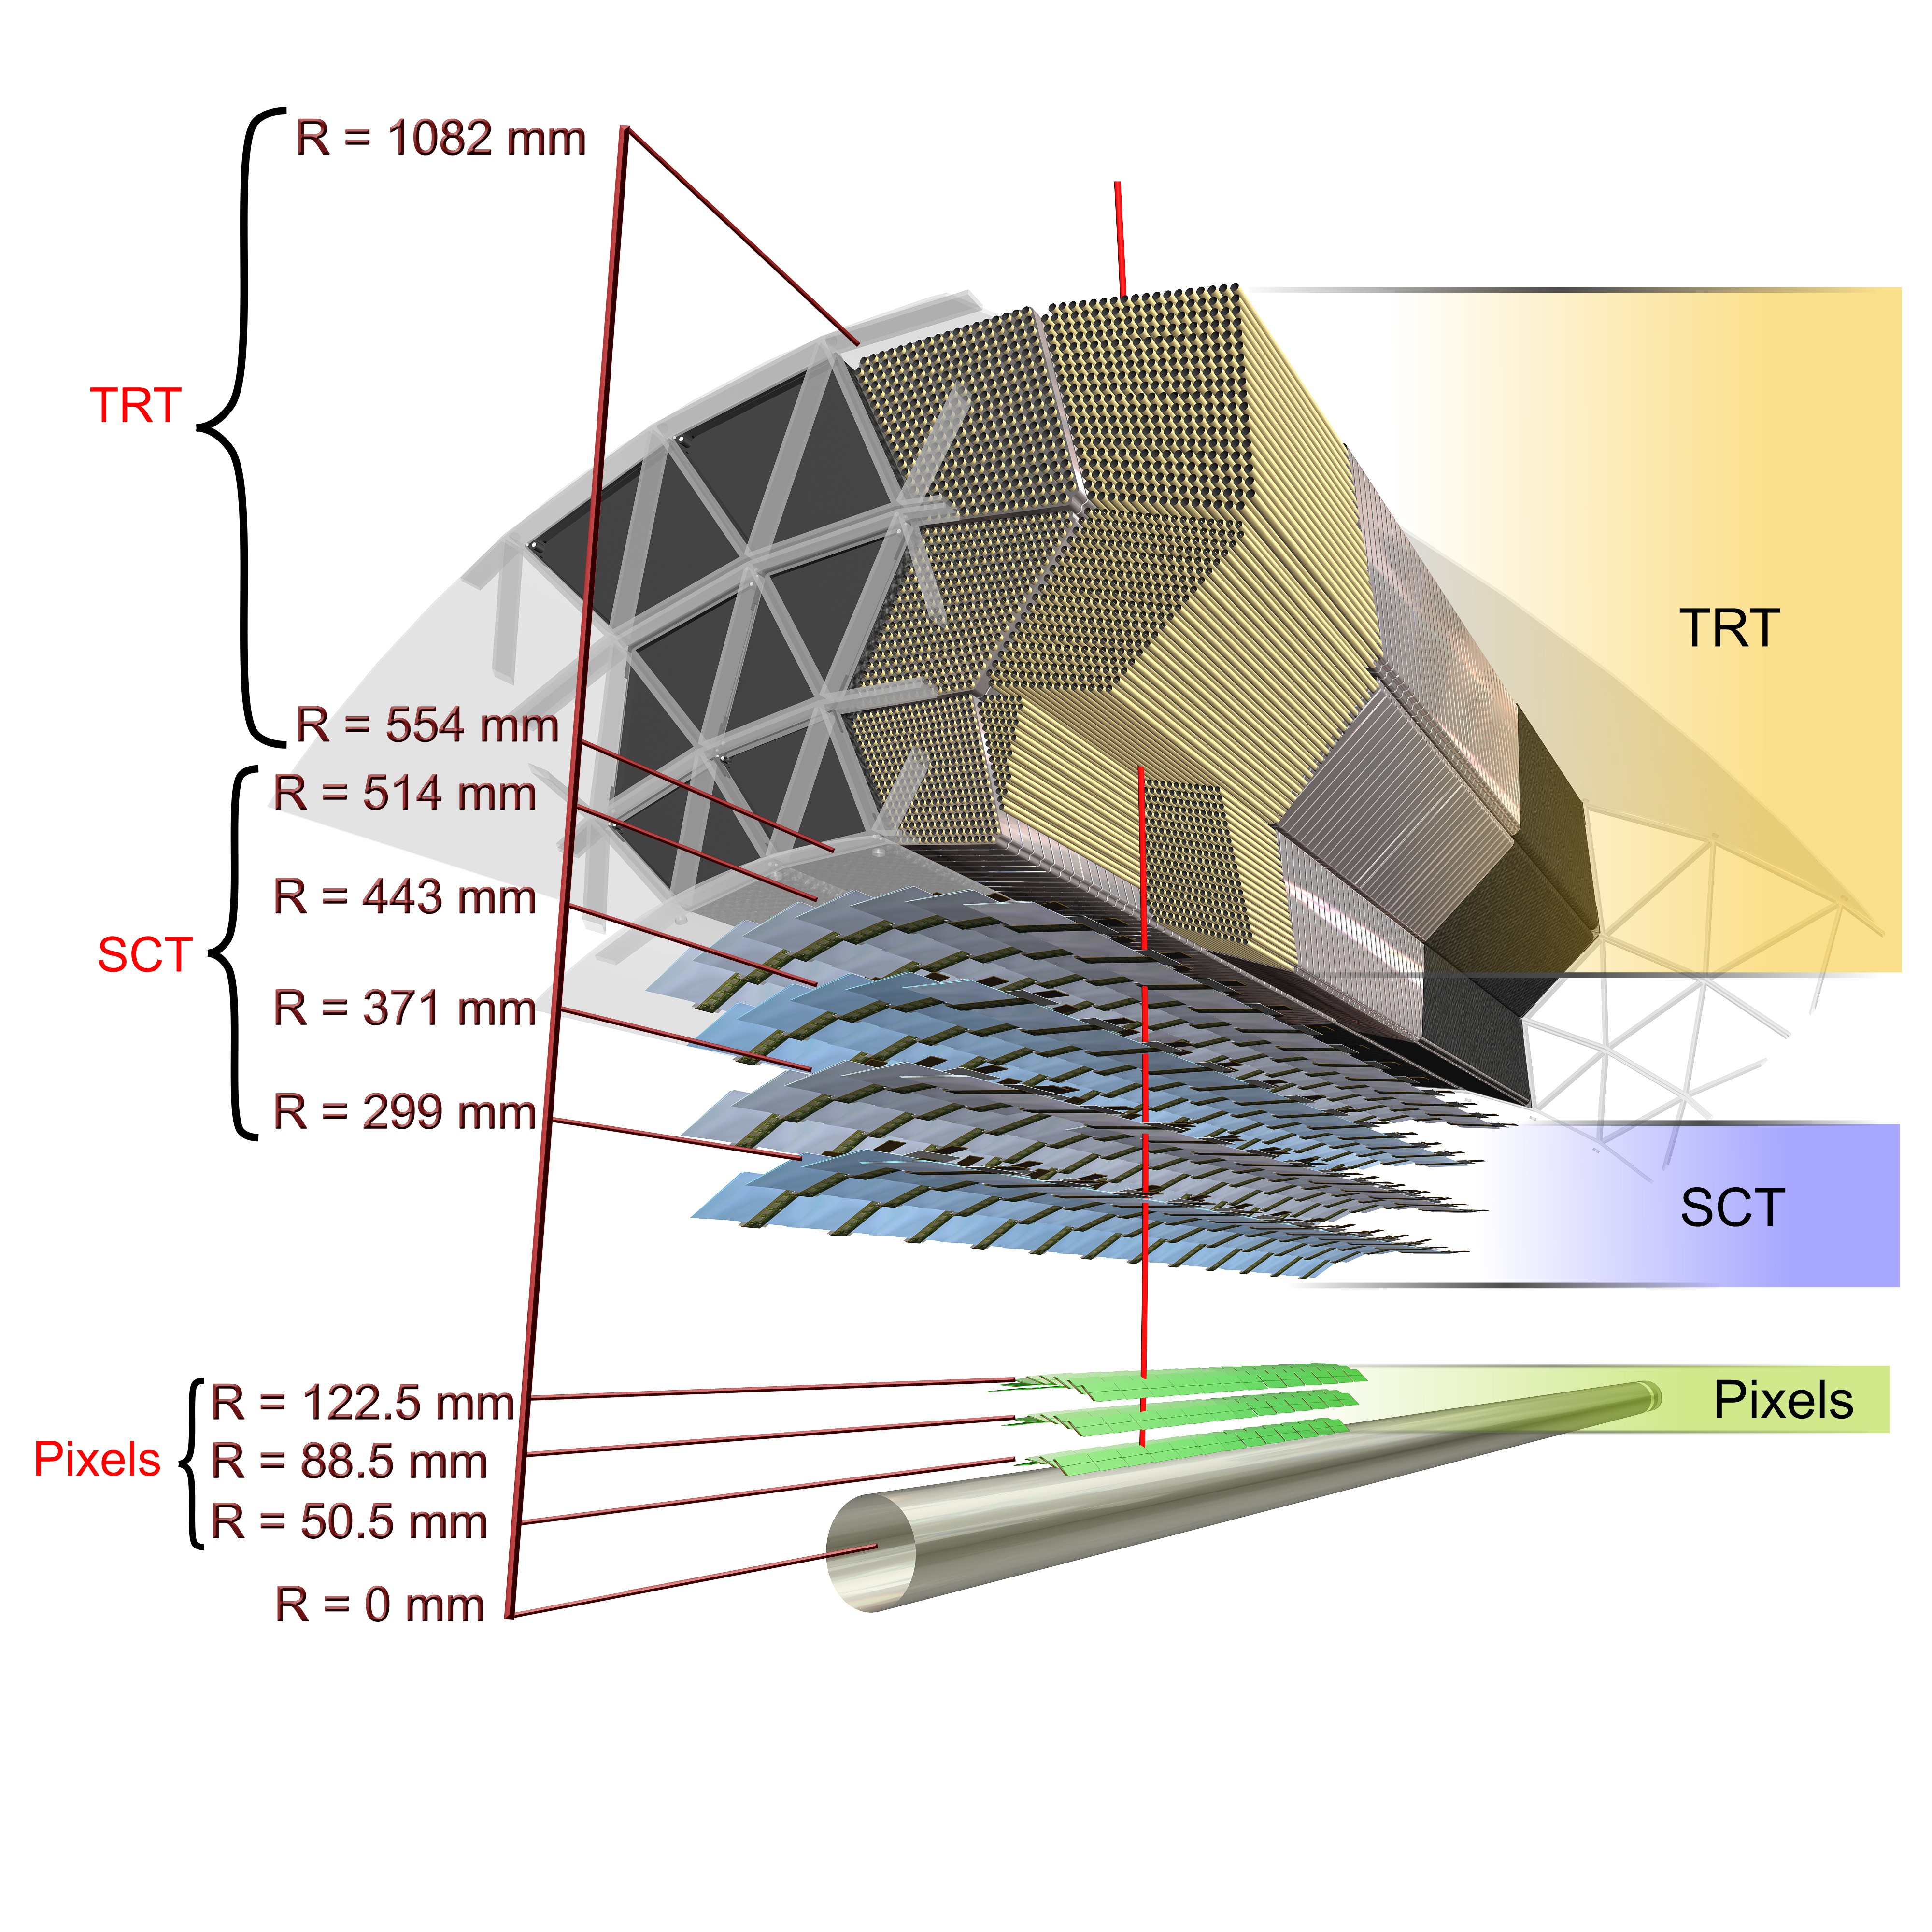
\includegraphics[width=0.7\textwidth]{inner-detector-2.jpg}
\label{fig:detector:inner-detector-2}
\caption{A cut-out view of the ATLAS inner detector, showing the layers a particle would interact with as it passed outward from the collision point. Copyright CERN.}
\end{figure}

%%%%%%%%%%%%%%%% 

\subsection{Silicon Pixel Detector}

The innermost ATLAS sub-detector is the Silicon Pixel Detector~\cite{ATLASPaper}. The principal of detection for the pixel detector follows the standard ionizing radiation detector~\cite{Detectors}. Charged particles interact with the active medium (doped silicon), knocking electrons loose from their host atoms and creating electron-hole pairs. An applied voltage carries the holes and electrons to opposite ends of the detectors, where they are read out. The active regions are very small in both $x$ and $y$ dimensions, allowing for many independent measurement channels in a small area. Given the high number of particles expected from LHC collisions, and that the density is greatest nearest to the interaction point, it is critical that the innermost detector have a huge number of very small channels, making the task perfectly suited for a pixel detector.

80.4 million independent pixel channels, with a size of $50 \times 400~\mu$m, are read out by 1744 bump-bonded modules attached to the active sensors. Each of the modules are composed of 16 front-end chips~\cite{ATLASPaper}. This corresponds to a combined active area of 1.7 $m^2$. The detector is arranged in three radial layers in the barrel section, and three disks in the end-caps. In the radial layers, the pixels have a resolution of $10 \times 115~\mu$m in $R-\phi$ and $z$ respectively, and in the end-caps the orientation is perpendicular and the resolution is $10 \times 115~\mu$m in $R$ and $R-\phi$: the orientations are always chosen such that the most precise measurement takes place in the direction most relevant to the measurement of the track $p_T$.\footnote{The $R-\phi$ coordinate is simply a distance-projected version of the azimuthal angle $\phi$.} The barrel and disk arrangement is shown in Figure~\ref{fig:detector:pixel}. Hits are read out when charge has been collected over a tunable threshold determined by the noise of each pixel, resulting in typical occupancies of $10^{-4}$ -- $10^{-5}$, though this grows obviously grows with additional $pp$ interactions.

The innermost radial layer, known as the $b$-layer, sits only 50.5 mm from the center of the beampipe, while the outermost layer is located at 122.5 mm~\cite{ATLASPaper}. By placing detectors so close to the interaction point, it is possible to very accurately measure the location of both  primary vertices-- the locations of $pp$ collisions-- and second vertices-- the locations of the displaced decays of particles with long lifetimes, such as $B$-hadrons~\cite{ATLASExpected}.

Placing the detector so close to the beamline comes at a price, however, as the detector is particularly susceptible to radiation damage due to the high flux of particles through a small area. At design luminosity, this is expected to be about 158 kGy/year at the $b$-layer, reduced to 25.4 kGy/year at the outermost layer~\cite{ATLASPaper}. Damage comes in the form of displaced atoms in the doped silicon lattice, resulting in lower electron-hole yields per particle interaction. Some of the damage is mitigated by operating at cold temperatures (typically $-5$ to $-10$\degree~C), and higher bias voltages can also alleviate the effects.

While the entire Inner Detector is expected to be replaced after 300 \ifb~are collected in order to replace the damaged components, the long shutdown of 2013-2015 presented ATLAS with the opportunity to augment the existing pixel detector with the so-called Insertable B-Layer (or IBL)~\cite{ATLASIBL}. The IBL, which adds an additional layer of pixels to the barrel and endcap pixel systems, is attached directly to a new carbon-fiber beampipe, and is located only 33 mm from the center of the beampipe. Due to this extremely close distance, the pixel size has been further reduced to $50 \times 250 \mu$m. The vertexing performance (especially secondary vertex identification for $b$-tagging) of ATLAS in Run 2, starting in 2015, is expected to substantially increase due to the IBL. 

%%%%%%%%%%%%%%%%

\begin{figure}
\centering
\includegraphics[width=0.7\textwidth]{pixel.jpg}
\label{fig:detector:pixel}
\caption{A computer-generated view of the ATLAS pixel detector. Copyright CERN.}
\end{figure}

%%%%%%%%%%%%%%%% 



\subsection{Silicon Strip Tracker}

The next outermost subdetector in the ID is composed of silicon microstrip (SCT) layers~\cite{ATLASPaper}. 


%%%%%%%%%%%%%%%%

\begin{figure}
\centering
\includegraphics[width=0.7\textwidth]{sct.jpg}
\label{fig:detector:sct}
\caption{A photograph of one segment of the ATLAS SCT end-cap disks. Copyright CERN.}
\end{figure}

%%%%%%%%%%%%%%%% 

\subsection{Transition Radiation Tracker}

%%%%%%%%%%%%%%%%

\begin{figure}
\centering
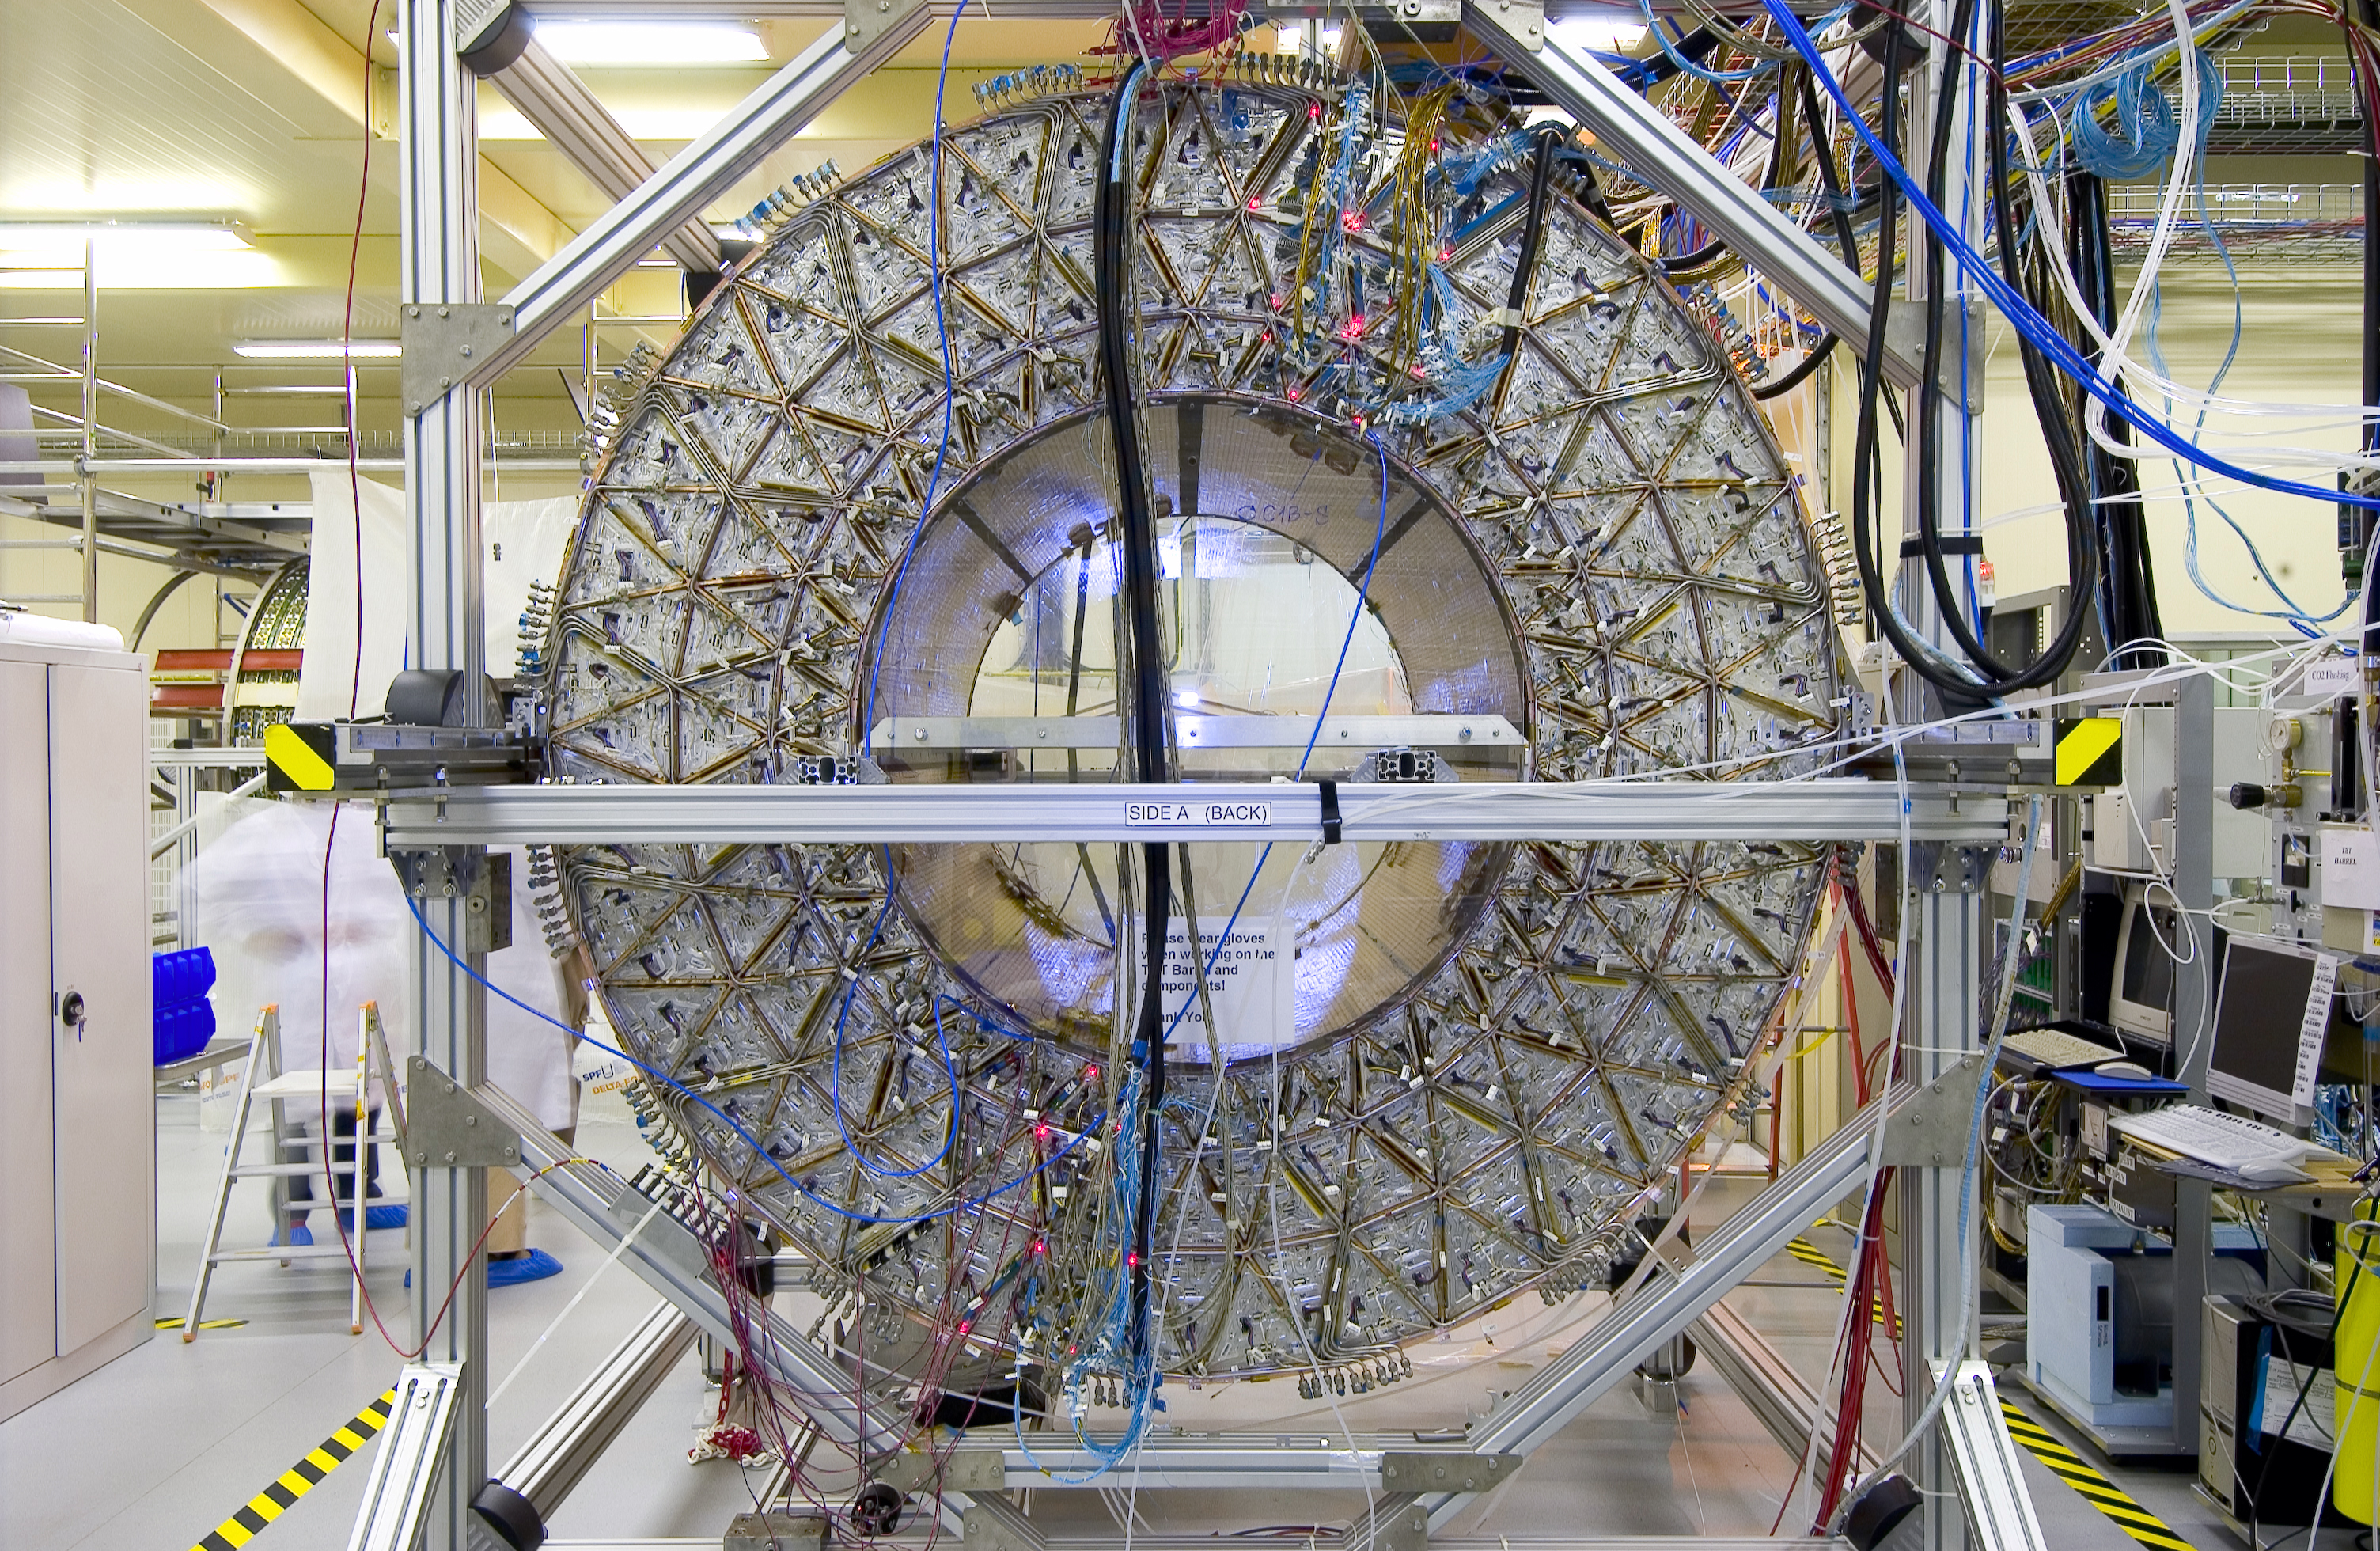
\includegraphics[width=0.7\textwidth]{trt.jpg}
\label{fig:detector:trt}
\caption{A photograph of the ATLAS TRT system during testing. Copyright CERN.}
\end{figure}

%%%%%%%%%%%%%%%% 

\section{Calorimeters}

%%%%%%%%%%%%%%%%

\begin{figure}
\centering
\includegraphics[width=0.7\textwidth]{calorimeters.jpg}
\label{fig:detector:trt}
\caption{A computer generated image of the ATLAS calorimeter system, showing the locations of each different subdetector. Copyright CERN.}
\end{figure}

%%%%%%%%%%%%%%%% 


\subsection{Electromagnetic Calorimeter}

%%%%%%%%%%%%%%%%

\begin{figure}
\centering
\includegraphics[width=0.7\textwidth]{lar-accordion.jpg}
\label{fig:detector:trt}
\caption{A photograph of the accordion structure used in the LAr barrel. Copyright CERN.}
\end{figure}

%%%%%%%%%%%%%%%% 

%%%%%%%%%%%%%%%%

\begin{figure}
\centering
\includegraphics[width=0.7\textwidth]{lar-endcap.jpg}
\label{fig:detector:trt}
\caption{A photograph of the LAr endcap after installation in the cryostat system. Copyright CERN.}
\end{figure}

%%%%%%%%%%%%%%%% 

\subsection{Hadron Calorimeter}

%%%%%%%%%%%%%%%%

\begin{figure}
\centering
\includegraphics[width=0.7\textwidth]{tile-actualtile.jpg}
\label{fig:detector:trt}
\caption{A photograph of one of the scintillating tiles which give the tile calorimeter its name. Copyright CERN.}
\end{figure}

%%%%%%%%%%%%%%%% 

%%%%%%%%%%%%%%%%

\begin{figure}
\centering
\includegraphics[width=0.7\textwidth]{tile.jpg}
\label{fig:detector:trt}
\caption{A photograph of the installation of the barrel tile calorimeter. Copyright CERN.}
\end{figure}

%%%%%%%%%%%%%%%% 


\section{Muon Spectrometer}


%%%%%%%%%%%%%%%%

\begin{figure}
\centering
\includegraphics[width=0.7\textwidth]{muons.jpg}
\label{fig:detector:trt}
\caption{A computer generated image showing the locations of each of the muon spectrometer subsystems. Copyright CERN.}
\end{figure}

%%%%%%%%%%%%%%%% 

\section{Triggering}

\section{Data Quality}


\chapter{Measuring Jets with ATLAS}
		...

\chapter{An Overview of Jet Substructure}
		...

\chapter{Seeing Color at the LHC}
		...

\chapter{Searching for Supersymmetry with Super Jets}
		...


\chapter{Conclusions}
         ...
\appendix
\chapter{A Long Proof}
         ...
\bibliographystyle{atlasBibStyleWithTitle}
\bibliography{swiatlow_thesis}
\end{document}